\documentclass[10pt]{article}
% -------------------------------------------------------------------
% Pacotes básicos
\usepackage[brazil]{babel}										% Idioma a ser usado
                                                                % Trocar "english" para "brazil" para artigos escritos em língua portuguesa 
\usepackage[utf8]{inputenc}										% Escrita de caracteres acentuados e cedilhas - 1
\usepackage[T1]{fontenc}										% Escrita de caracteres acentuados + outros detalhes técnicos fundamentais
% -------------------------------------------------------------------
% Pacotes matemáticos
\usepackage{amsmath,amsfonts,amssymb,amsthm,cancel,siunitx,
calculator,calc,mathtools,empheq,latexsym}
% -------------------------------------------------------------------
% Pacotes para inserção de figuras e subfiguras
\usepackage{subfig,epsfig,tikz,float}		            % Packages de figuras. 
% -------------------------------------------------------------------
% Pacotes para inserção de tabelas
\usepackage{booktabs,multicol,multirow,tabularx,array}          % Packages para tabela
% -------------------------------------------------------------------
\usepackage{float}
\usepackage{biblatex}
\usepackage[colorlinks=true, allcolors=blue]{hyperref}
\usepackage{lipsum}
\usepackage{listings} % for code
% trying to How can one keep a \section from being at the end of a page?
% \usepackage[nobottomtitles*]{titlesec}

% -------------------------------------------------------------------
% Definition of lengths
\setlength{\parskip}{5pt}
\textwidth 13.5cm
\textheight 19.5cm
\columnsep .5cm
% -------------------------------------------------------------------
% Title of the Article
\title{\renewcommand{\baselinestretch}{1.17}\normalsize\bf%
\uppercase{Flutter Canteen}
}
% -------------------------------------------------------------------
% Authors
\author{%
  Almeida, João\\
  \texttt{a2020144466@isec.pt}
  \and
  Afonso, Kylix\\
  \texttt{a2020146228@isec.pt}
  \and
  Oliveira, Rafaela\\
  \texttt{a2019127935@isec.pt}
}
% -------------------------------------------------------------------

% Begin Document

\begin{document}

\date{\today}

\maketitle

\vspace{-0.5cm}

\begin{center}
{\footnotesize 
ISEC Coimbra, Dept. de Engenharia Informática e Sistemas \\
}
\end{center}

% -------------------------------------------------------------------
% Abstract
\bigskip
\noindent
\begin{abstract}
    Este projeto tem como objetivo criar uma aplicação para visualização e gestão dos menus semanais de uma cantina. A aplicação permite que os usuários visualizem os menus disponíveis e façam pedidos de mudança. Também permite que os usuários tirem fotos dos seus pratos e as envie para serem adicionadas ao catálogo, utilizando tecnologias integradas com flutter que permitem acesso à câmara e à localização a partir de dispositivos móveis.
%	\lipsum[2-4]
\end{abstract}

\medskip
\noindent
%{\small{\bf Keywords}{:} 
%computer vision, tensorflow, classification, raspberry pi, python, object detection, %machine learning, opencv
%}

\baselineskip=\normalbaselineskip

\pagebreak
\tableofcontents
\pagebreak
% -------------------------------------------------------------------

\section{Introdução}\label{sec:1}

Este relatório tem como objetivo apresentar o processo de desenvolvimento de uma aplicação desenvolvida em Flutter, uma plataforma de desenvolvimento de aplicações móveis que permite criar aplicações para iOS e Android com uma única base de código. 

A aplicação em causa tem como principal objetivo oferecer aos usuários a possibilidade de visualizar os menus semanais da cantina e fazer pedidos de alteração, além de permitir que os usuários tirem fotos de seus pratos e as enviem para atualizar o catálogo. 

Neste relatório, vamos analisar o design da interface da aplicação, a abordagem e arquitetura utilizadas, bem como a integração de tecnologias como a comunicação com o servidor, a utilização da câmara, o acesso à localização e coordenadas e o uso de dados locais através de shared preferences. Também discutiremos brevemente os desafios encontrados durante o desenvolvimento da aplicação e as lições aprendidas.

\pagebreak

\section{Análise do design da interface}\label{sec:2}

    A aplicação consiste apenas em dois ecrãs, Um ecrã principal com informação geral sobre as refeições e um ecrã de detalhes de cada dia.
    O tempo gasto não foi muito focado no embelezamento da interface, mas foram tomados os passos necessários para que esta fosse intuitiva e não tivesse qualquer problema relativamente à interação e à mostra da informação. 

	\begin{figure}[H]
		\centering
		\begin{minipage}[b]{0.32\textwidth}
			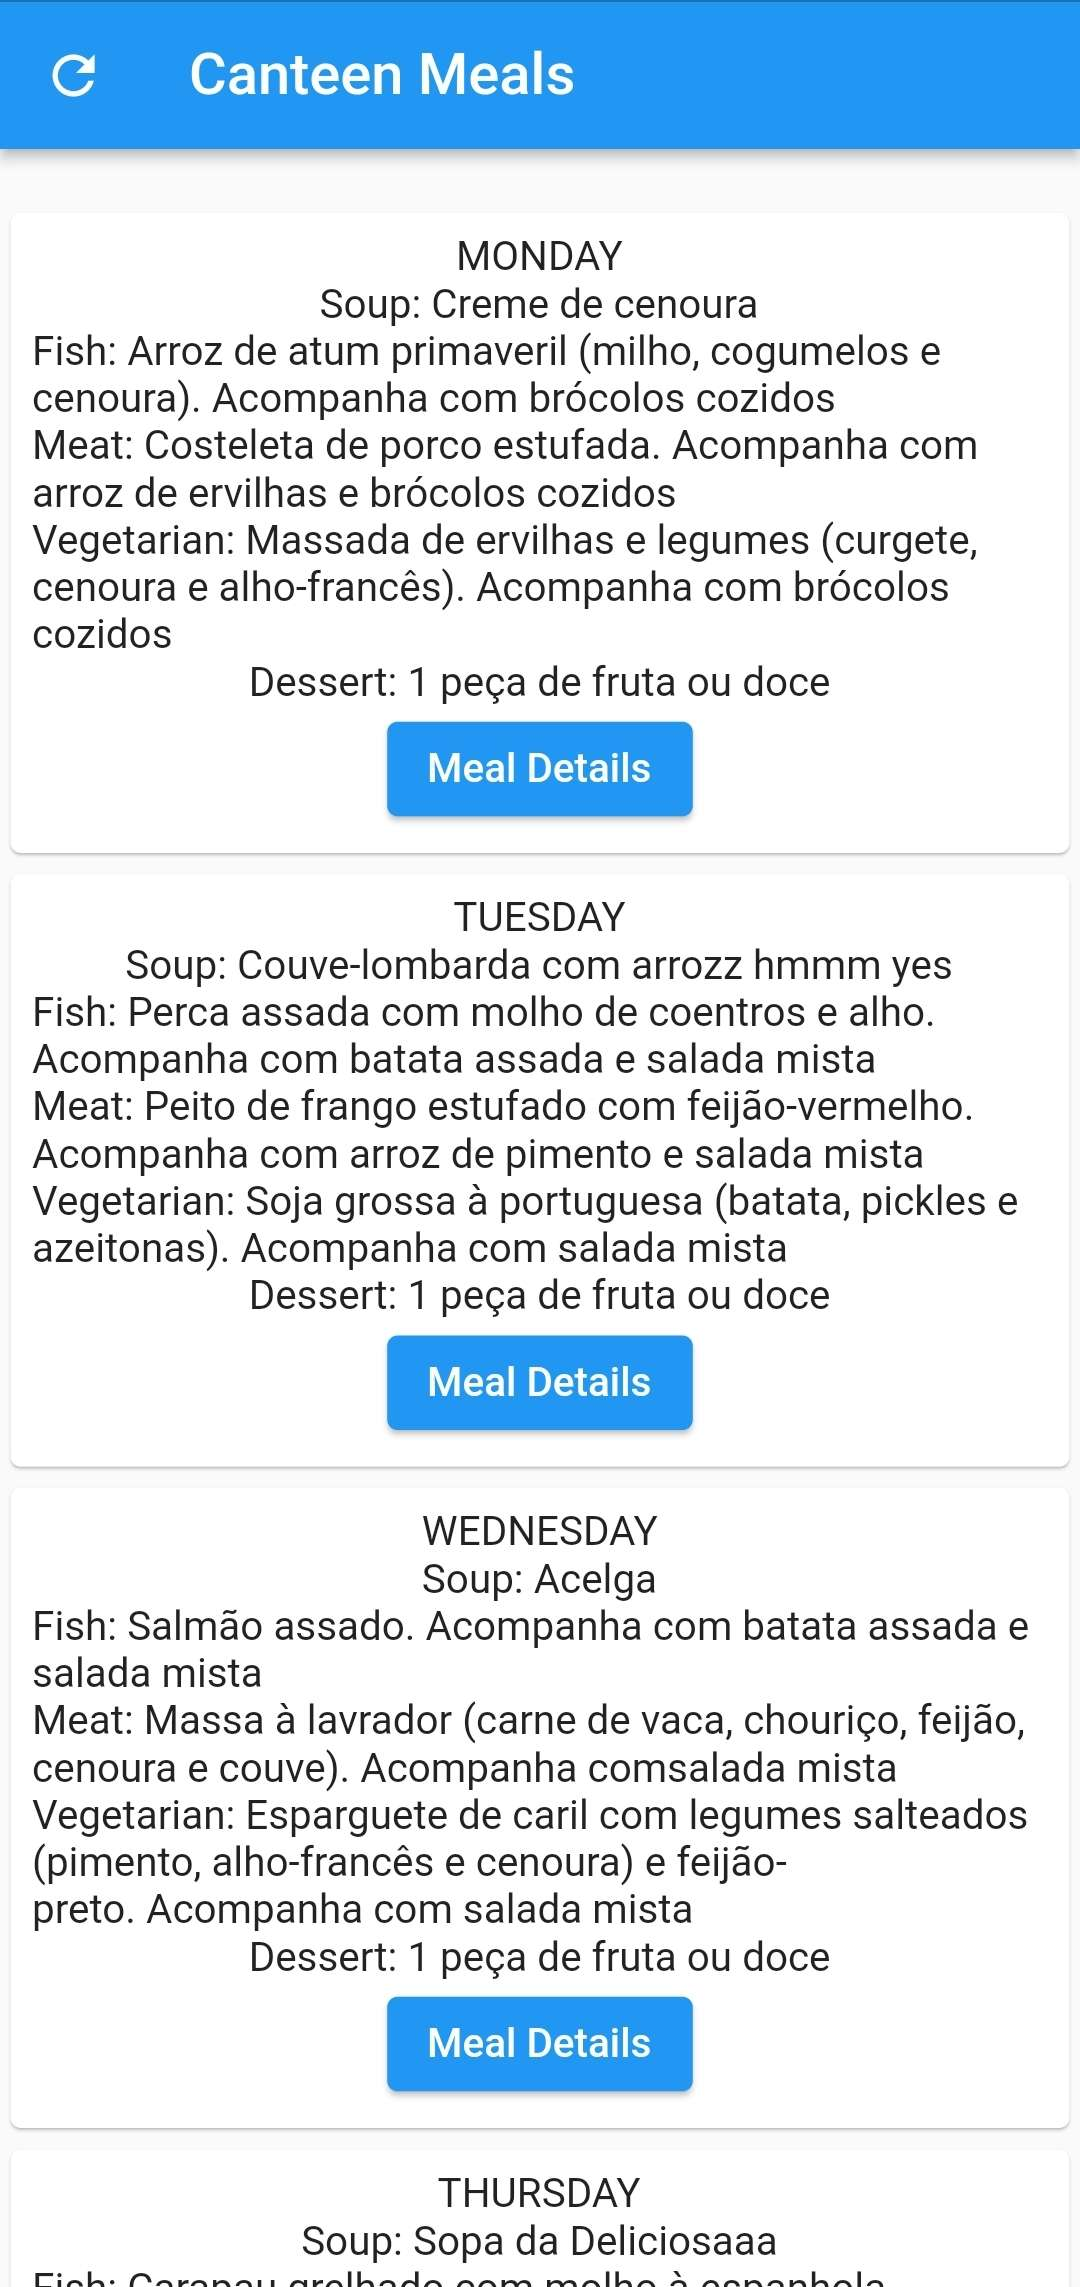
\includegraphics[width=\textwidth]{imgs/main_menu.jpg}
			\caption{Ecrã Principal}
		\end{minipage}
		\hfill
		\begin{minipage}[b]{0.32\textwidth}
			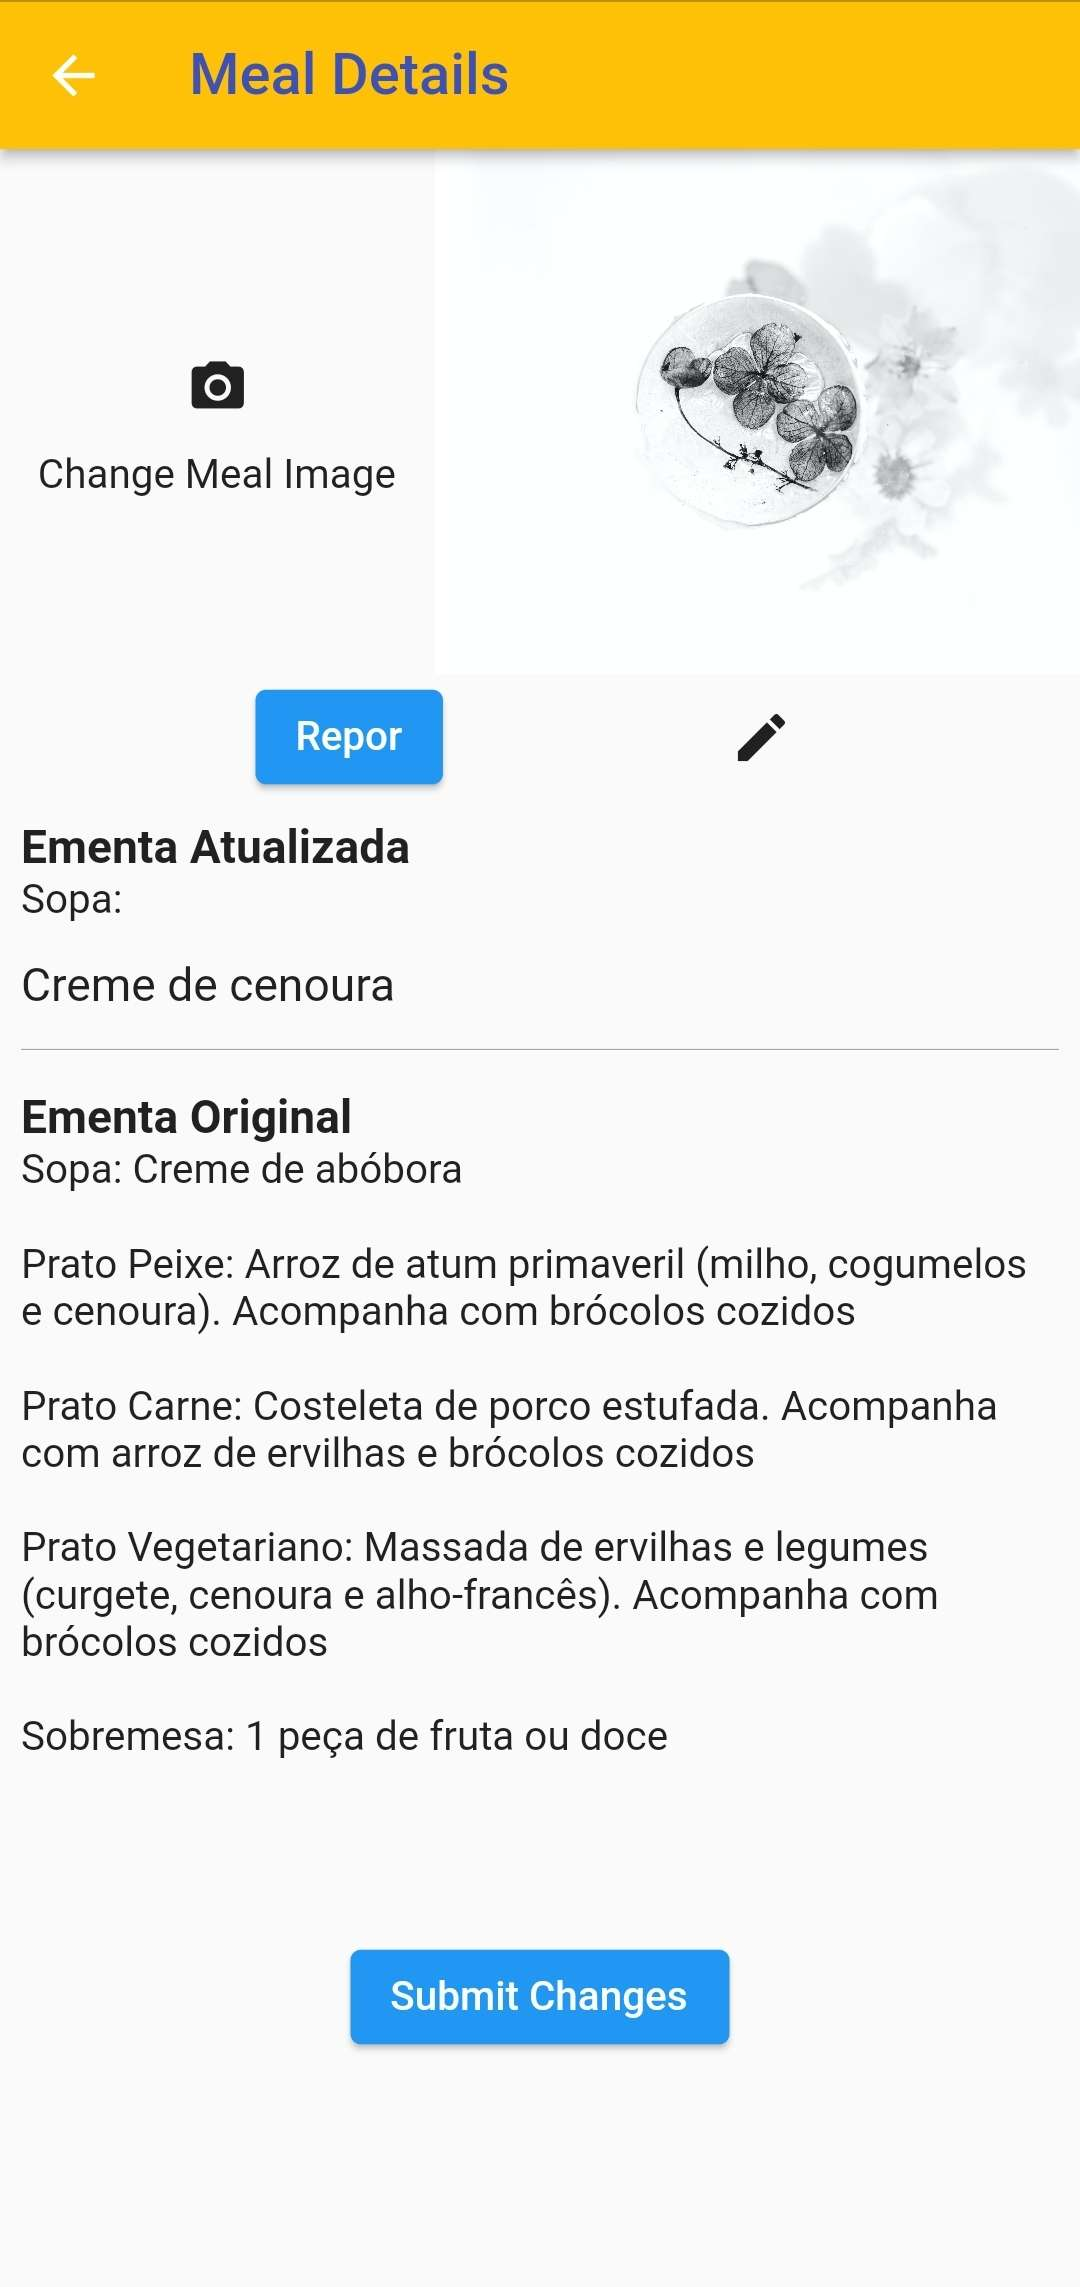
\includegraphics[width=\textwidth]{imgs/meal_details}
			\caption{Ecrã dos Detalhes da Refeição (com imagem por defeito)}
		\end{minipage}
	\end{figure}

    \subsection{Ecrã Principal}

    Este ecrã terá uma lista infinita que mostra a informação atualizada de cada ementa de cada dia, começando pelo dia da semana em que o utilizador se encontra no acesso, caso não haja informação atualizada por qualquer utilizador, será mostrada a informação original do servidor.

    A informação está guardada localmente, e é apenas atualizada quando o utilizador pressiona o botão de refresh em cima à esquerda (ou quando submete uma alteração a uma refeição). A informação localmente guardada será falada mais em detalhe na secção dos \nameref{shared_preferences}

    \subsection{Ecrã dos Detalhes da Refeição}

    Neste ecrã é mostrado ao utilizador a foto associada à refeição, seja ela a original, uma atualizada, ou uma por defeito caso nenhuma destas exista, bem como onformação atualizada e original sobre a ementa.

    Há também um botão para editar a informação, um botão para repor toda a informação, incluindo a imagem, e um botão para tirar uma foto.

    O utilizador poderá alterar a foto, e a informação, mas a informação só será atualizada se após isso pressionar o botão "Submit Changes" e se encontrar a no mínimo 1Km da cantina do ISEC.

    Devido à utilização da camara e da localização, ambas estas premissões são pedidas ao utilizador ao entrar neste ecrã.

\section{Abordagem e Arquitetura}\label{sec:3}

	\subsection{Tools}

		Como já mencionado, a tecnologia usada foi o Flutter, e o foco foi numa aplicação móvel para android.

        Foi também necessário instalar um ambiente onde fosse possivel correr o servidor dado em docker para se ter acesso ao servidor. No entanto teve-se em conta as alterações feitas no servidor do professor na última semana, pelo que o trabalho que entregamos comunica diretamente com o servidor do professor: \href{http://amov.servehttp.com:8080/menu}{http://amov.servehttp.com:8080/menu}.

        Outras packages de Flutter\cite{1} usadas incluem:

        \begin{itemize}
		\item http, to communicate with the server
		\item shared\_preferences, to store the information locally
		\item location, to access the device location
		\item camera, to allow taking photos
            \item latlong2, to facilitate coordinates manipulation
	\end{itemize}

    \pagebreak

        \subsection{Estrutura de Ficheiros}

        Para além da estrutura criada pelas ferramentas usadas, dividimos o projeto em três ficheiros: main.dart, meal\_details.dart, constants.dart. Se foi feita a dedução de que o ficheiro main.dart foi usado para o ecrã principal e o ficheiro meal\_details foi usado para o ecrã de detalhes de refeições, a dedução estaroia correta.

        Foi criado também um ficheiro para constantes que acabou por ter apenas informação sobre o site onde se vai buscar a informação, pelo que a única informação que consta deste ficheiro é a seguinte:
        \begin{lstlisting}
const String SERVER_URL = 'http://amov.servehttp.com:8080';
        \end{lstlisting}
        Esta linha poderá ser fácilmente mudada para rápidamente mudar o servidor.

 
	\subsection{Comunicação com o Servidor}

        A informação é obtida com o get request desta forma:

        \begin{lstlisting}[language=Dart]
http.Response response = await http.get(Uri.parse(_serverMenuUrl));
        \end{lstlisting}

        Para postar informação, é feito atraves de um post comn toda a informação relevante da seguinte forma:

        \begin{lstlisting}[language=Dart]
  final uri = Uri.parse('${constants.SERVER_URL}/menu');
  final response = await http.post(
    uri,
    headers: <String, String>{
      'Content-Type': 'application/json; charset=UTF-8',
    },
    body: jsonEncode(
        {
          "img": imgBase64new,
          "weekDay": updatedMeal.weekDay,
          "soup": updatedMeal.updatedSoup,
          "fish": updatedMeal.updatedFish,
          "meat": updatedMeal.updatedMeat,
          "vegetarian": updatedMeal.updatedVegetarian,
          "desert": updatedMeal.updatedDessert,
        }),
  );
        \end{lstlisting}

        Atenção que a imagem obtida da câmara é convertida para Base64 primeiro para poder ser interpretada pelo servidor.

        \subsection{Utilização da Câmara}

        A utilização da câmara resume-se à sua inicialização e à utilização do método takePicture() para tirar uma foto quando o icon da câmara é pressionado.

        De seguida é executado um setState() para colocar a imagem visivel na interface.
        
        \subsection{Acesso a localização e coordenadas}

        O utilizador pode apenas submeter alterações às refeições da cantina se se encontrar a menos de um kilometro desta. Para este fim é utilizado o plugin location para obter as coordenadas do dispositivo e o plugin latlong2 para as tratar. 

        Se o utilizador se encontrar a mais de um kilometro da cantina, é mostrado um erro ao tentar submeter com a distância que o utilizador se encontra da cantina.

        \pagebreak

        \subsection{Dados locais (shared\_preferences)}\label{shared_preferences} 
        

		A aplicação irá comunicar com o servidor apenas quando expressamente pedido pelo utilizador, mostrando apenas a informação localmente guardada em qualqeur outra situação atravez do plugin das shared\_preferences.
        Caso não haja qualquer informação para mostrar, o utilizador é informado.

	\begin{figure}[H]
		\centering
		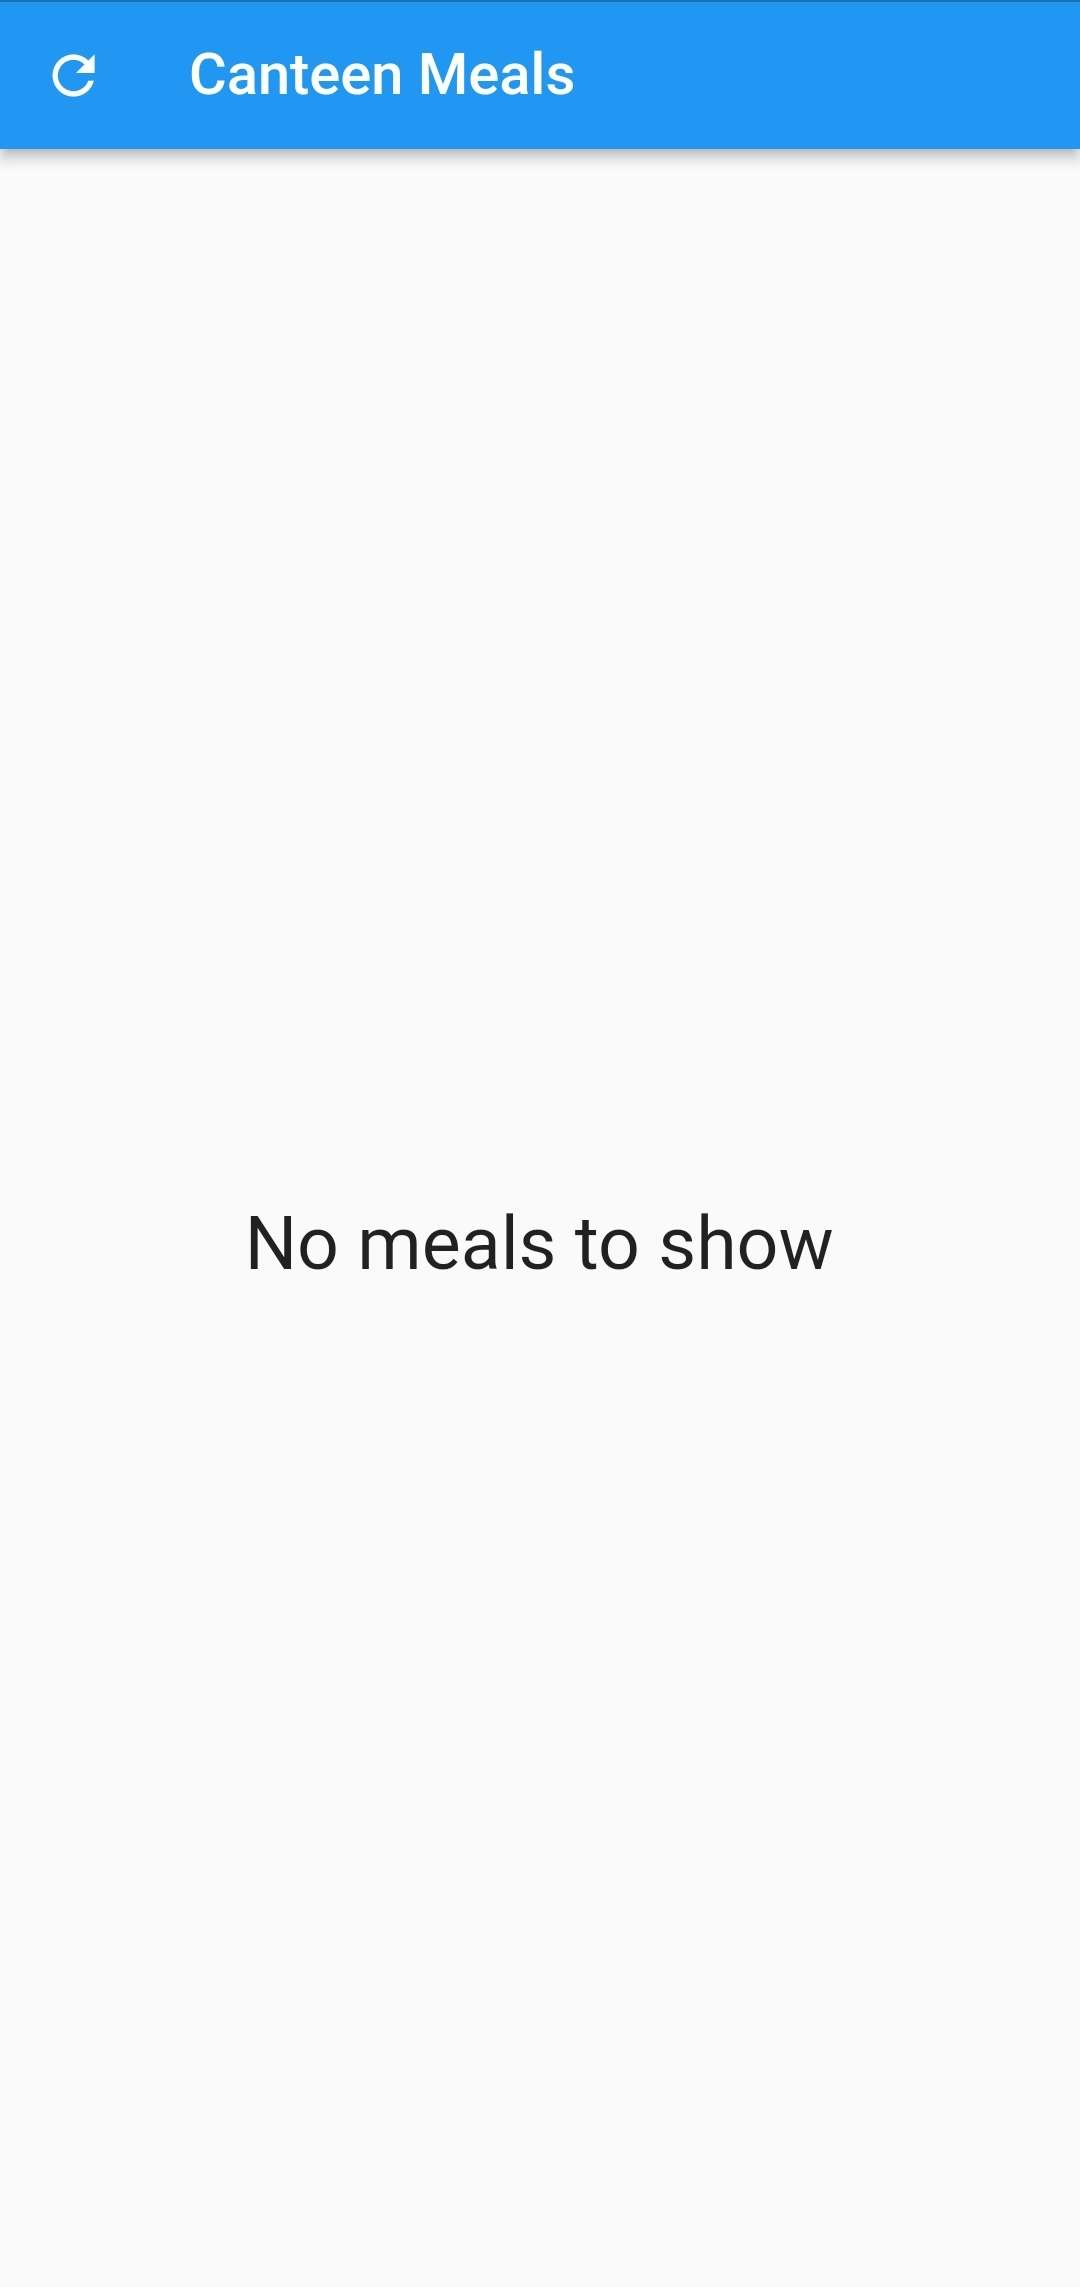
\includegraphics[scale=0.10]{imgs/no_meals_to_show.jpg}
		\caption{Screen when there are no meals to show locally stored}\label{fig:usage}
	\end{figure}

 São usadas as seguintes funções para guardar a obter informação:

\begin{lstlisting}[language=Dart]
static Future<bool> saveMeals(Uint8List mealzz) async {
    final SharedPreferences prefs = await SharedPreferences.getInstance();
    String base64Image = base64Encode(mealzz);
    return prefs.setString("storedMeals", base64Image);
}

static Future<Uint8List> getMeals() async {
    final SharedPreferences prefs = await SharedPreferences.getInstance();
    Uint8List bytes = base64Decode(prefs.getString("storedMeals") ?? '');
    return bytes;
}
\end{lstlisting}
 

\section{Conclusão} 

 	Foi-nos possível completar todas as tarefas propostas a este trabalho, bem como as opcionais, na sua totalidade.

  Achamos que o balnço deste trabalho é positivo, pelo que aprendemos a usar uma das tecnologias mais relevantes da ária, uma vez que nos permite lançar uma aplicação para variados dispositivos e sistemas operativos com apenas uma base de código.


% There is a better way to do the bibliography for sure
\begin{thebibliography}{1}
	\bibitem{1}
	\href{https://pub.dev}{The official package repository for Dart and Flutter apps.}

	\bibitem{2}
	\href{https://stackoverflow.com}{A private collaboration & knowledge sharing platform.}
\end{thebibliography}

\end{document}